\documentclass[11pt,a4paper]{article}

\usepackage[margin=1in]{geometry}
\usepackage[utf8]{inputenc}
\usepackage[T1]{fontenc}
\usepackage{lmodern}
\usepackage{amsmath,amssymb,amsthm,mathtools}
\usepackage{microtype}
\usepackage{booktabs}
\usepackage{graphicx}
\usepackage{array}
\usepackage{xcolor}
\usepackage{hyperref}
\usepackage{longtable}
\usepackage{float}
\usepackage{caption}
\usepackage{subcaption}
\usepackage{enumitem}

\newtheorem{theorem}{Theorem}[section]
\newtheorem{definition}[theorem]{Definition}
\newcommand{\eps}{\varepsilon}
\newcommand{\dimH}{\dim_{\mathrm H}}
\newcommand{\dimB}{\dim_{\mathrm B}}

\title{\textbf{Dimensions of Strange Attractors}}
\author{Filip Nowakowicz}

\begin{document}
\maketitle

\tableofcontents
\newpage

\section{Dimensions of sets}

\begin{definition}[Box-counting dimension]
	Let \(Z\subset \mathbb R^m\) be bounded. Let \(N(Z,\eps)\) be the smallest number of balls of radius \(\eps\) needed to cover \(Z\). The lower and upper box dimensions are
	\[
		\underline{\dim}_{\mathrm B} Z
		= \liminf_{\eps\to 0}\frac{\log N(Z,\eps)}{-\log \eps},
		\qquad
		\overline{\dim}_{\mathrm B} Z
		= \limsup_{\eps\to 0}\frac{\log N(Z,\eps)}{-\log \eps}
	\]
	If \(\underline{\dim}_{\mathrm B} Z = \overline{\dim}_{\mathrm B} Z\), the common value is the box-counting dimensions \(\dim_{\mathrm B} Z\).
\end{definition}

The box-counting dimension can be easily computed dimensionally, however, it only sees the support, which means that a dense region will count equally as a rarely visited one.

\begin{definition}[Hausdorff dimension]
	Given \(s\geq 0\), the \(s\)-dimensional Hausdorff measure is defined by
	\[
		\mathcal{H}^s(Z)
		= \lim_{\delta\to 0}
		\inf\left\{\sum_i (\openratorname{diam} U_i)^s:
		Z\subset \bigcup_i U_i,\ \openratorname{diam} U_i<\delta\right\}
	\]
	Hausdorff dimension is the critical value of \(s\)
	\[
		\dimH Z = \inf\{s: \mathcal{H}^s(Z)=0\}
		= \sup\{s: \mathcal{H}^s(Z)=\infty\}
	\]
\end{definition}
Hausdorff dimension is more rigorous and captures geometric scaling, but it is more difficult to estimate numerically. It can be bounded above by the following inequality.
\[
	\dimH Z \leq \underline{\dim}_{\mathrm B} Z
	\leq \overline{\dim}_{\mathrm B} Z
\]
The issue with considering set dimensionality is that a subset of phase space only considers the attractor's support and not the underlying distribution of the orbits inside that set. This motivates the next chapter.

\section{Dimensions of measures}

For a chaotic system, one can analyse invariant probability measures supported on the attractor to get statistically relevant objects.

\begin{definition}[Hausdorff dimension of a measure]
	Let \(\mu\) be a finite Borel measure on a metric space \(X\).
	\[
		\dimH \mu
		= \inf\{\dimH Z: \mu(X\setminus Z)=0\}
	\]
\end{definition}

The following two dimensions are especially significant for numerical approximations.

\begin{definition}[Information dimension]
	For a partition of space into boxes of size \(\eps\), let \(p_i(\eps)\) be the mass of the \(i\)-th box. The information dimension is morally
	\[
		D_1(\mu)
		= \lim_{\eps\to0}
		\frac{-\sum_i p_i(\eps)\log p_i(\eps)}{-\log \eps},
	\]
	when the limit exists.
\end{definition}

\begin{definition}[Correlation dimension]
	\[
		C(r) = \int \mu(B(x,r))\,d\mu(x),
		\qquad
		D_2(\mu)=\lim_{r\to 0}\frac{\log C(r)}{\log r}.
	\]
	\noindent For a finite orbit sample \(x_1,\dots,x_N\), the following numerical approximation can be used.
	\[
		C_N(r)=\frac{1}{N(N-1)}\#\{(i,j):i\neq j,\ d(x_i,x_j)<r\}.
	\]
\end{definition}
\noindent Correlation dimension counts pairs of points in an orbit that are closer than \(r\) to each other, which unlike the box-counting dimension, makes it dependent on the distribution of points in an orbit.

The notion of the dimension of a measure can be extended by considering the dimension of local neighbourhoods of points in \(X\), which results in a curve of dimensions.
\begin{definition}[Pointwise dimension]
	The pointwise or local dimension of \(\mu\) at \(x\) is
	\[
		d_\mu(x)
		= \lim_{r\to 0}\frac{\log \mu(B(x,r))}{\log r},
	\]
	if the limit exists.
\end{definition}
\noindent Intuitively, if \(\mu(B(x,r)) \approx r^{d_\mu(x)}\) for small \(r\), then the smaller the local dimension, the more concentrated the mass is near \(x\).
% The change in dimension motivates the study of the \(\alpha\)-level sets
% \[
%     E(\alpha)=\{x:d_\mu(x)=\alpha\}
% \]
% The multifractal spectrum is defined by
% \[
%     f(\alpha)=\dimH E(\alpha)
% \]
\begin{definition}[Exact dimensionality]
	A measure is exact dimensional if there exists \(d\) such that
	\[
		d_\mu(x)=d
	\]
	for \(\mu\)-almost every \(x\).
\end{definition}

\begin{theorem}[Young's dimension criterion, simplified]
	Suppose \(\mu\) is a \emph{exact dimensional} finite measure on a metric space and
	for \(\mu\)-almost every \(x\). Then the natural dimensions of \(\mu\) coincide and equal \(d\).
	\[
		\dimH \mu = \underline{\dim}_{\mathrm B} \mu = \overline{\dim}_{\mathrm B} \mu = d
	\]
\end{theorem}

This criterion is useful when showing a physical measure is exact dimensional, since the values of local dimensions should concentrate around the same value.

\section{Invariant, ergodic, and physical measures}

\begin{definition}[Invariant measure]
	Let \((X,\mathcal{B})\) be a measurable space and \(f:X\to X\) measurable. A probability measure \(\mu\) is \(f\)-invariant if
	\[
		\mu(f^{-1}A)=\mu(A)
	\]
	for every measurable set \(A\)
\end{definition}

\noindent The distribution of points is unchanged by applying the dynamics.

A dynamical system is called ergodic if every invariant measurable set has measure either \(0\) or \(1\). % Measure-preserving systems

\begin{theorem}[Birkhoff ergodic theorem]
	Let \(f:X\to X\) be a measurable map such that \(\mu\) is invariant with respect to \(f\), and let \(\varphi\in L^1(\mu)\). Then the time averages
	\[
		\frac1n\sum_{k=0}^{n-1}\varphi(f^k x)
	\]
	converge for \(\mu\)-almost every \(x\). If \(\mu\) is ergodic, then the limit is
	\[
		\int \varphi\,d\mu
	\]
	for \(\mu\)-almost every \(x\).
\end{theorem}
Birkhoff's egodic theorem relates the average behaviour along a single trajectory to the space average of the whole system. This justifies considering only a single long orbit during numerical estimations.

\begin{definition}[Physical measure]
	For a probability measure \(\mu\), define its basin by
	\[
		B(\mu)=\left\{x : \frac{1}{n}\sum_{k=0}^{n-1}\varphi(f^k x)
		\to \int \varphi\, d\mu
		\text{ for } \varphi \in C^0(X) \right\} %Observables
	\]
	A probability measure \(\mu\) is called a physical measure if \(B(\mu)\) has positive Lebesgue measure.
\end{definition}
\noindent Physical measures ensure that they describe the behaviour from a positive-volume set of initial conditions, which means its physically observable.

\section{SRB measures}

SRB (Sinai--Ruelle--Bowen) measures are a class of invariant probability measures used to describe the statistical behaviour of chaotic systems with hyperbolic behaviour. \\
Consider the follow decomposition of a hyperbolic system on an invariant set.
\[
	T_xM = E_x^s \oplus E_x^u
\]
where vectors in \(E_x^s\) contract under forward iteration and vectors in \(E_x^u\) expand under forward iteration.
If the space is restricted to two dimensions \(M = \mathbb R^2\), then \(T_xM \cong \mathbb R^2\), hence
\[
	\mathbb R^2 = E_x^s \oplus E_x^u
\]
An SRB measure is a physical and invariant measure that is absolutely continuous with respect to Lebesgue measure along unstable directions, while singular along stable directions.

These measures are important as they describe the statistical behaviour from a set of initial conditions with a positive Lebesgue measure. For many chaotic systems with strange attractors, trajectories starting from such initial conditions exhibit converging behaviours described by an SRB measure. This allows us to connect this concept with physical quantities such as entropy and Lyapunov exponents.

\section{Lyapunov exponents}

\begin{definition}[Lyapunov exponents]
	For a differentiable map \(f:M\to M\), Lyapunov exponents represent the exponential growth rates of tangent vectors.
	\[
		\lambda(x,v)
		= \lim_{n\to\infty}\frac1n\log\|D_xf^n v\|,
	\]
	when the limit exists.
\end{definition}
\begin{theorem}[Oseledets' theorem, schematic]
	Let \(f\) preserve an ergodic probability measure \(\mu\), and assume suitable regularity conditions. Then for \(\mu\)-almost every \(x\), there exist Lyapunov exponents
	\[
		\lambda_1 > \lambda_2 > \cdots > \lambda_k
	\]
	and an invariant decomposition
	\[
		T_xM = E_1(x)\oplus \cdots \oplus E_k(x)
	\]
	such that vectors in \(E_i(x)\) grow or contract exponentially at rate \(\lambda_i\):
	\[
		\|Df^n(x)v\| \approx e^{\lambda_i n}
		\quad \text{for } v \in E_i(x)
	\]
\end{theorem}

\begin{definition}[Kaplan--Yorke dimension]
	Let the Lyapunov exponents be ordered
	\[
		\lambda_1\geq \lambda_2\geq\cdots\geq \lambda_m
	\]
	Let \(j\) be the largest integer such that
	\[
		\sum_{i=1}^j \lambda_i \geq 0
	\]
	The Kaplan--Yorke dimension is
	\[
		D_{\mathrm{KY}}
		= j+\frac{\sum_{i=1}^j\lambda_i}{|\lambda_{j+1}|}
	\]
\end{definition}
\noindent In a two-dimensional space with \(\lambda_1 > 0 > \lambda_2\) this simplifies to the following.
\[
	D_{\mathrm{KY}} = 1 + \frac{\lambda _1}{|\lambda _2|}
\]
This can be understood as the expanding direction contributing one full dimension, since its absolutely continuous in that subspace, while the stable direction produces a fractional part. This results in the dimension being the balance between stretches and contractions in the system. Unlike the other dimensions, this one is directly motivated by the dynamics and not the underlying geometric complexities. This concept can be generalised by considering the entropy of the system.

\section{Entropy}

Metric Entropy is the average rate at which the information about the system is lost under iteration, or equivalently, it is the measure of unpredictability of a dynamical system.
For sufficiently smooth hyperbolic systems, the statistical complexity is directly related to dynamical instability through Pesin's entropy formula.
\begin{theorem}[Pesin entropy formula]
	For sufficiently smooth hyperbolic systems and an SRB measure \(\mu\),
	\[
		h_\mu(f)=\sum_{\lambda_i>0}\lambda_i m_i,
	\]
	where \(h_\mu(f)\) is metric entropy, \(\lambda_i\) are Lyapunov exponents, and \(m_i\) are their multiplicities.
\end{theorem}
The above results above suggest a relation between the dimension of an invariant measure, the complexity of the system, and the Lyapunov exponents. In particular, the entropy is determined by the positive Lyapunov exponents.

Ledrappier--Young theory provides a more rigorous relation between entropy and dimensions. For an ergodic hyperbolic invariant measure, the dimension can be decomposed along invariant subspaces.
\[
	T_xM = E_1(x)\oplus\cdots\oplus E_k(x)
\]
Each invariant subspace contributes a partial dimension \(\delta_i\), such that
\[
	\dim \mu = \sum_i \delta_i
\]
These partial dimensions are determined by entropy levels in a given subspace divides by the corresponding Lyapunov exponent.
\[
	\delta_i = \frac{h_i-h_{i-1}}{\lambda_i},
\]
where \(h_i-h_{i-1}\) is the entropy contribution associated with the \(i\)-th Lyapunov direction.

\noindent This simplifies in the two-dimensional hyperbolic case, where
\[
	\mathbb R^2 = E_x^u \oplus E_x^s,
	\qquad
	\lambda_u > 0 > \lambda_s,
\]
the dimension decomposes into unstable and stable contributions,
\[
	\dim \mu = \delta_u + \delta_s,
\]
where
\[
	\delta_u = \frac{h_\mu(f)}{\lambda _u},
	\qquad
	\delta_s = \frac{h_\mu(f)}{|\lambda _s|},
\]
For an two-dimensional SRB measure, Pesin's formula gives \(h_\mu(f) = \lambda_u\), which agrees with the Kaplan--Yorke dimension, since this implies that \(\delta_u =1\) and \(\delta_s = \frac{\lambda _u}{|\lambda _s |}\).
While in two dimensions the reduction is simple, in higher-dimensional systems the Ledrappier--Young theory provides a richer understanding of dimensions.

\section{Numerical investigation of the H\'enon map}

H\'enon map is described by the following equation.
\[
	H_{a,b}(x,y)=(1-a x^2+y,\ bx)
\]
with the standard parameter values
\[
	a=1.4, \qquad b=0.3
\]

The computation uses a single orbit after discarding the given number of initial points.  The empirical measure is
\[
	\mu_N=\frac1N\sum_{i=1}^N\delta_{z_i},
	\qquad z_i=H_{a,b}^i(z_0)
\]

\subsection{Lyapunov exponents and the Kaplan--Yorke estimation}

For the H\'enon map, the Jacobian matrix is
\[
	DH_{a,b}(x,y)=
	\begin{pmatrix}
		-2ax & 1 \\
		b    & 0
	\end{pmatrix}
\]
The Lyapunov exponents were estimated by iterating this Jacobian along the orbit and applying QR re-orthonormalisation. Let \(Q_n\) is an orthonormal basis, one computes
\[
	DH_{a,b}(z_n)Q_n = Q_{n+1}R_n,
\]
and estimates
\[
	\lambda_i \approx \frac1N\sum_{n=1}^N \log |(R_n)_{ii}|
\]
This method simplifies the complexity of multiplying many Jacobian matrices directly

The resulting exponents were
\[
	\lambda_1\approx 0.42018,
	\qquad
	\lambda_2\approx -1.62415
\]
Since \(\lambda_1>0>\lambda_2\), the Kaplan--Yorke dimension is
\[
	D_{\mathrm{KY}}
	=1+\frac{0.42018}{1.62415}
	\approx 1.25871
\]

\subsection{Dimension comparison}

Three additional dimensiowhenns were estimated numerically. The box-counting estimation used the slope of
\[
	\log N(\eps) \quad \text{against} \quad \log(1/\eps),
\]
where \(N(\eps)\) is the number of occupied grid boxes. The information estimation used the slope of
\[
	-\sum_i p_i(\eps)\log p_i(\eps) \quad \text{against} \quad \log(1/\eps),
\]
The correlation estimator used the slope of
\[
	\log C_N(r) \quad \text{against} \quad \log r.
\]

\begin{table}[H]
	\centering
	\begin{tabular}{lcc}
		\toprule
		Quantity           & Estimate & 95\% bootstrap interval \\
		\midrule
		$D_{KY}$           & $1.259$  & n/a                     \\
		$D_{\mathrm{box}}$ & $1.245$  & $[1.235,1.256]$         \\
		$D_2$              & $1.202$  & $[1.196,1.207]$         \\
		$D_1$              & $1.229$  & $[1.222,1.238]$         \\
		\bottomrule
	\end{tabular}
	\caption{Global dimensions for the H\'enon map at $a=1.4$, $b=0.3$.}
	\label{tab:global-dimensions}
\end{table}

The estimates are not equal but they consistently approximate a value around or above \(1.2\). This is expected as each method focused on slightly different aspects to calculate the dimension.

The 95\% intervals were computed by bootstrap resampling of the points, which means that the points were sampled with replacement, the regression slope was refitted, and the appropriate percentiles of the results were recorded.


% A bootstrap resampling method is used to produce the confidence intervals. Lyapunov exponents were estimated by iteratively applying the Jacobian of the H\'enon map to an orthonormal basis and then applying the QR decomposition.

\subsection{Generalised dimensions}

To see how the dimension changes as denser regions receive more weight, I estimated the generalised R\'enyi dimensions \(D_q\).
\begin{definition}[Generalised dimensions]
	Let \(\mu\) be a probability measure on \(\mathbb R^m\). For \(\eps>0\), partition \(\mathbb R^m\) into boxes of side length \(\eps\), and let \(p_i(\eps)\) be the \(\mu\)-mass of the \(i\)-th box. For \(q\neq 1\), the generalised dimension of order \(q\) is
	\[
		D_q(\mu)
		=
		\lim_{\eps\to 0}
		\frac{1}{q-1}
		\frac{\log \sum_i p_i(\eps)^q}{\log \eps},
	\]
	whenever the limit exists.

	\noindent For \(q=1\), it is the information dimension.
\end{definition}

\begin{table}[H]
	\centering
	\begin{tabular}{rcc}
		\toprule
		$q$   & $D_q$   & 95\% bootstrap interval \\
		\midrule
		$0$   & $1.245$ & $[1.234,1.257]$         \\
		$0.5$ & $1.241$ & $[1.234,1.249]$         \\
		$1$   & $1.229$ & $[1.222,1.238]$         \\
		$1.5$ & $1.213$ & $[1.205,1.223]$         \\
		$2$   & $1.191$ & $[1.179,1.202]$         \\
		$3$   & $1.123$ & $[1.102,1.144]$         \\
		$4$   & $1.048$ & $[1.013,1.079]$         \\
		\bottomrule
	\end{tabular}
	\caption{Generalised dimension estimates $D_q$.}
	\label{tab:generalised-dimensions}
\end{table}

\begin{figure}[H]
	\centering
	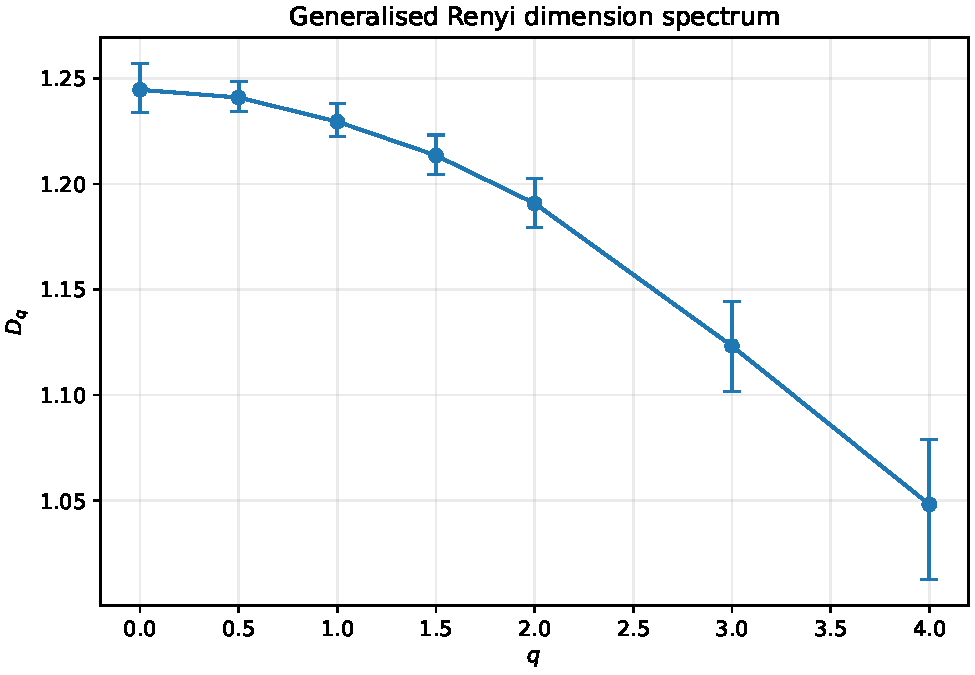
\includegraphics[width=0.78\textwidth]{figures/generalized_dimension_spectrum.pdf}
	\caption{Estimated generalised dimension spectrum.}
	\label{fig:generalized-spectrum}
\end{figure}
The numerical results show a monotone decreasing trend. Larger \(q\) gives more weight to boxes with large mass, so the result suggests that the empirical measure is not distributed uniformly on its support.

\subsection{Local dimensions and exact-dimensionality}

For a point \(x\) on the orbit, the local dimensions was estimated by
\[
	\log\mu_N(B(x,r))\quad \text{against}\quad \log r.
\]
A standard approach of plotting a fixed set of small value of \(r\) did not produce correct results, which is why I shifted to using a \(k\)-nearest-neighbour version. Let \(r_k(x)\) be the distance from \(x\) to its \(k\)-th nearest neighbour, then
\[
	\mu_N(B(x,r_k(x)))\approx \frac{k}{N}
\]
Thus a local dimension estimate comes from fitting
\[
	\log(k/N) \quad \text{against} \quad \log r_k(x)
\]
For each orbit length, \(N\), I sampled 500 points and for each point I used 18 logarithmically spaced \(k\)s between \(k_{\min}\approx N^{0.25}\) and \(k_{\max}\approx N^{0.70}\). Each point is then one local dimension estimate. The 95\% interval was calculated by resampling the 500 point estimated with replacement and recomputing the mean for each bootstrap sample and taking the relevant percentiles of the means.

\begin{table}[H]
	\centering
	\begin{tabular}{rcccc}
		\toprule

		$N$       & mean    & 95\% mean interval & std. dev. & IQR     \\
		\midrule
		$50000$   & $1.266$ & $[1.244,1.288]$    & $0.248$   & $0.296$ \\
		$100000$  & $1.250$ & $[1.232,1.269]$    & $0.214$   & $0.258$ \\
		$300000$  & $1.244$ & $[1.229,1.261]$    & $0.191$   & $0.214$ \\
		$1000000$ & $1.247$ & $[1.231,1.262]$    & $0.171$   & $0.172$ \\
		\bottomrule
	\end{tabular}
	\caption{Local dimension estimates for increasing orbit length.}
	\label{tab:local-N}
\end{table}

\begin{figure}[H]
	\centering
	\begin{subfigure}{0.49\textwidth}
		\centering
		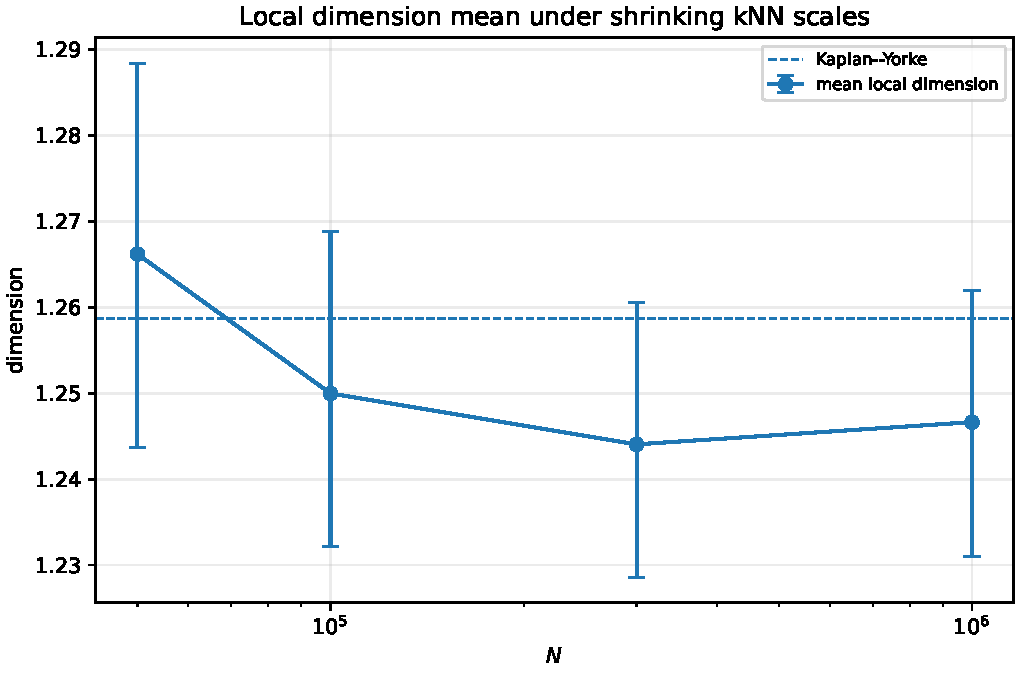
\includegraphics[width=\textwidth]{figures/local_dimension_mean_vs_N.pdf}
		\caption{Mean local dimension.}
	\end{subfigure}
	\hfill
	\begin{subfigure}{0.49\textwidth}
		\centering
		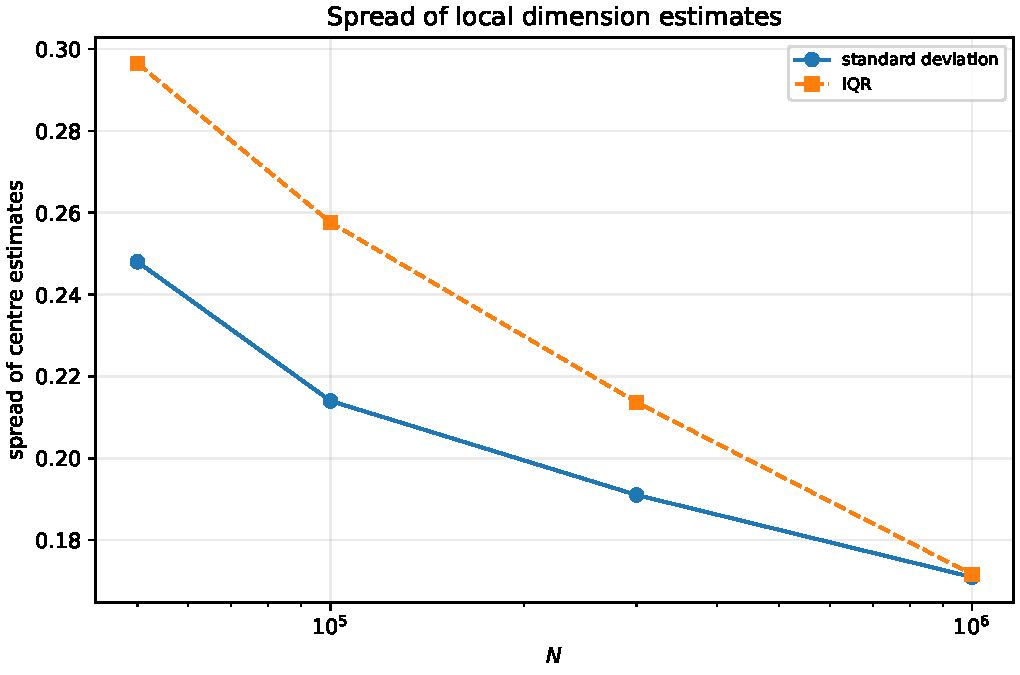
\includegraphics[width=\textwidth]{figures/local_dimension_spread_vs_N.pdf}
		\caption{Spread of centre estimates.}
	\end{subfigure}
	% \caption{The shrinking \(k\)-nearest-neighbour diagnostic keeps the mean close to the global dimension estimates while the spread decreases.}
	\label{fig:local-knn}
\end{figure}

The mean stays close to the global dimension estimates as $N$ increases while the spread decreases, which suggests an exact dimensional behaviour.

\subsection{Random petrubations WIP / SKIP}

The investigation considered a peturbed H\'enon system to simulate noise.
\[
	x_{n+1} = f(x_n) + \sigma \zeta_n,
\]
where \(\zeta _n\) is sampled uniformly from the unit disk, while \(\sigma\) controls the amplitude of the noise.
The experiment used $N=100000$ and 500 local dimension estimates for each noise level. The results are shown in Table \ref{tab:sigma}.

\begin{table}[H]
	\centering
	\begin{tabular}{rcccc}
		\toprule
		$\sigma$ & mean    & median  & std. dev. & IQR     \\
		\midrule
		$0$      & $1.239$ & $1.243$ & $0.228$   & $0.297$ \\
		$0.0001$ & $1.245$ & $1.230$ & $0.244$   & $0.319$ \\
		$0.0005$ & $1.276$ & $1.268$ & $0.220$   & $0.288$ \\
		$0.001$  & $1.262$ & $1.245$ & $0.222$   & $0.283$ \\
		$0.002$  & $1.283$ & $1.266$ & $0.206$   & $0.292$ \\
		$0.003$  & $1.336$ & $1.318$ & $0.227$   & $0.299$ \\
		$0.004$  & $1.372$ & $1.357$ & $0.212$   & $0.269$ \\
		$0.005$  & $1.421$ & $1.405$ & $0.202$   & $0.251$ \\
		\bottomrule
	\end{tabular}
	\caption{Local dimension estimates under increasing noise for $N=100000$.}
	\label{tab:sigma}
\end{table}
Clear increasing trend. Always converges to 2 but with different speed.


\end{document}
